\documentclass[a4paper]{article}

\usepackage[T2A]{fontenc}
\usepackage[utf8]{inputenc}
\usepackage[russian]{babel}

\usepackage[unicode, colorlinks, linkcolor=blue, citecolor=blue]{hyperref}
\usepackage{amsmath}
\usepackage{graphicx}
\graphicspath{{pictures/}}
\DeclareGraphicsExtensions{.pdf,.png,.jpg}

\usepackage{pgfplots}
\usepackage{tikz}

\usepackage[]{geometry}
\geometry
{
	a4paper,
	total={170mm,257mm},
	left=25mm,
	top=19mm,
	right=25mm
}

\begin{document}
	\selectlanguage{russian}
	%----------------------------------Шапка--------------------------------------
	\begin{figure}[htb]
		\begin{minipage}[c]{0.12\textwidth}
			
\includegraphics[scale=0.25]{AU}
		\end{minipage}
		\hfill
		\begin{minipage}[t]{0.9\textwidth}
			{\Large\bfseries Санкт-Петербургский национальный исследовательский Академический университет имени Ж.И.~Алфёрова\\Российской академии наук}
		\end{minipage}
		\rule{164mm}{0.3mm}
	\end{figure}
	
	\begin{center}
		{\large\textbf{Рабочий протокол и отчёт по лабораторной работе №3 }}\\
		Свиридов Фёдор, Александр Слободнюк, Владимир Попов
	\end{center}
	\begin{center}
		\Large\bfseries{<<Эффект Холла в примесном полупроводнике>>}\\
	\end{center}
	%-------------------------------------------------------------------------------
	
	{\parindent=0pt\textbf{Исходные данные.}}\\
	\begin{center}
		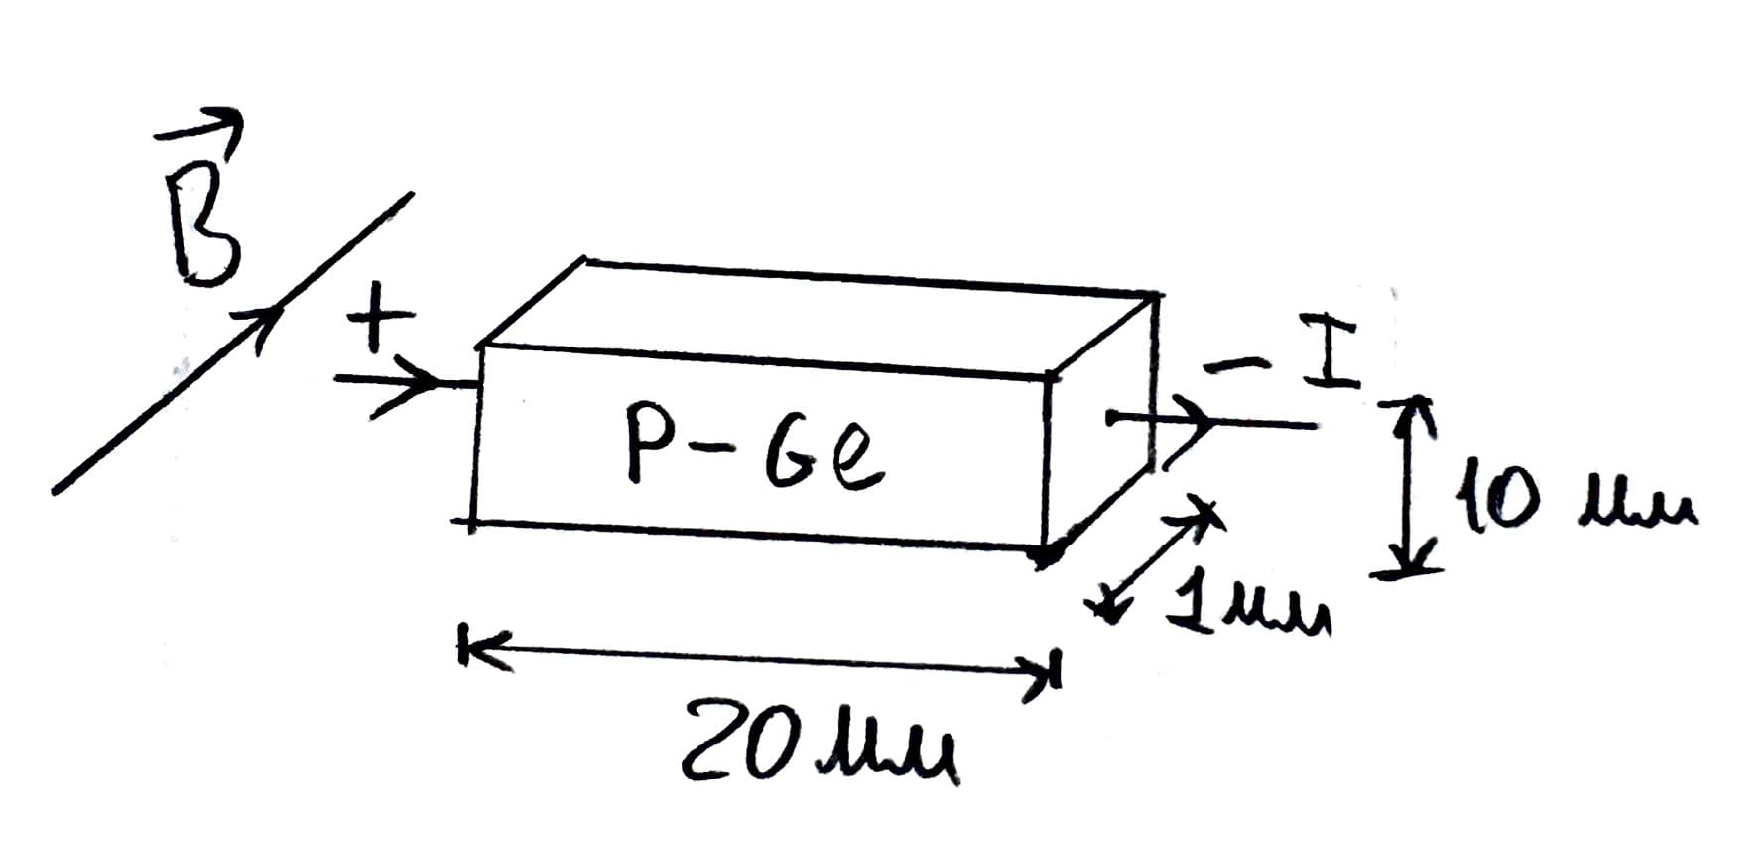
\includegraphics[scale=0.3]{pain}
	\end{center}
Геометрические размеры полупроводника p-Ge:
$l=20\;\mbox{мм}$; $h=10\;\mbox{мм}$; $d=1\;\mbox{мм}$; $S=hd=10\;\mbox{мм}^2$.
\begin{equation}
	I=\sigma\frac{S}{l}\,U_{\parallel}
\end{equation}

\begin{equation}
	U_{\perp}=R\frac{I}{d}\,B
\end{equation}

\begin{equation}
	R=\frac{1}{en}
\end{equation}
	
	
	{\parindent=0pt\textbf{Результаты прямых измерений.}}\\
	Вольт-амперная характеристика для полупроводника при нулевом магнитном поле:
	\begin{center}
	\begin{tabular}{c|c}
		\hline
		$I$, мА&$U_{\parallel}$, В  \\
		\hline
		5&0,22  \\
		10&  0,46\\
		15&  0,75\\
		20&  0,98\\
		25&  1,22\\
		30&  1,49\\
		35&  1,77\\
		40&  2,07\\
		
	\end{tabular}
\end{center}
Зависимость поперечного напряжения $U_{\perp}$ (ЭДС Холла) от силы магнитного поля
\begin{center}
	\begin{tabular}{c|c|c}
		\hline
		$I$, A&$B$, Тл  & $U_{\perp}$, В \\
		\hline
		0,0& 0,007 &  30,0\\
		0,2&  	0,014		&  30,8\\
		0,4&  	0,032		&  32,7\\
		0,6&  		0,056	& 35,4 \\
		0,8& 			0,080 & 38,2 \\
		1,0&  			0,103	&  40,7\\
		1,2&  			0,123	& 43,0 \\
		1,4&  		0,148	& 45,6 \\
		1,6&  			0,176& 48,5 \\
		1,8& 			 0,207&  51,7\\
		2,0& 				 0,222& 53,3 \\
	\end{tabular}
\end{center}

{\parindent=0pt\textbf{Обработка результатов и расчёт косвенных величин.}}\\
Экстраполяция ВАХ:
\begin{center}
	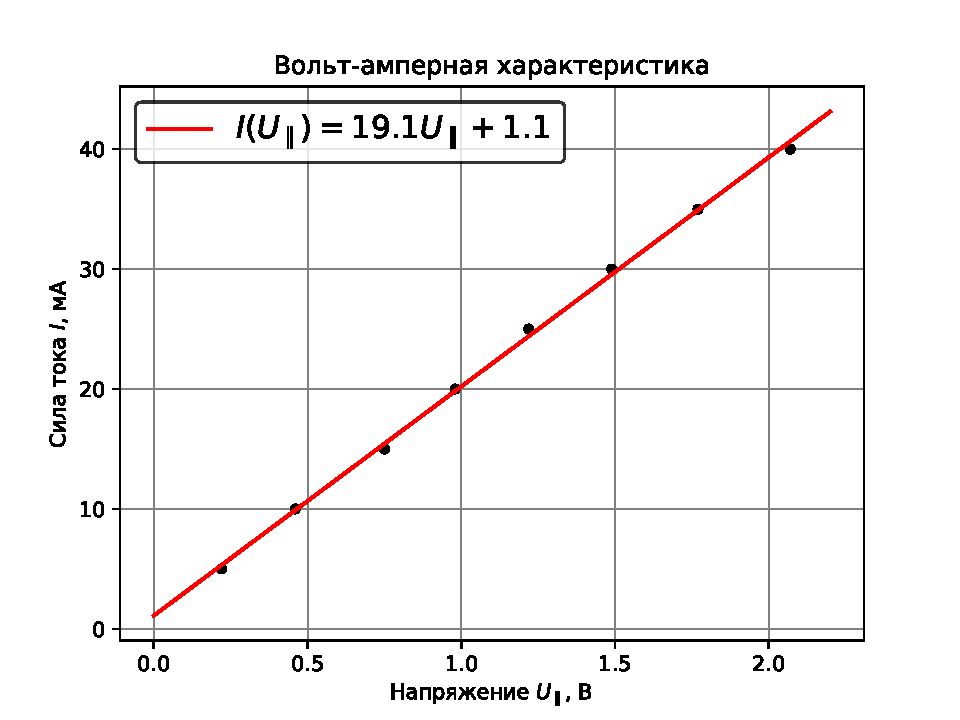
\includegraphics[scale=0.6]{BAX}
\end{center}

Из формулы (1) $k=\sigma\frac{S}{l}$, где $k=19.1\;\left( \frac{\mbox{мА}}{\mbox{В}}\right) $ - коэффициент пропорциональности ВАХ.\\
 Отсюда получаем: $\sigma=k\frac{l}{S}$
 $$ \sigma=19,1\cdot10^{-3}\cdot\frac{20\cdot10^{-3}}{10\cdot10^{-6}}=38,2\quad(\mbox{Ом}^{-1}\cdot\mbox{м}^{-1})$$

\begin{center}
	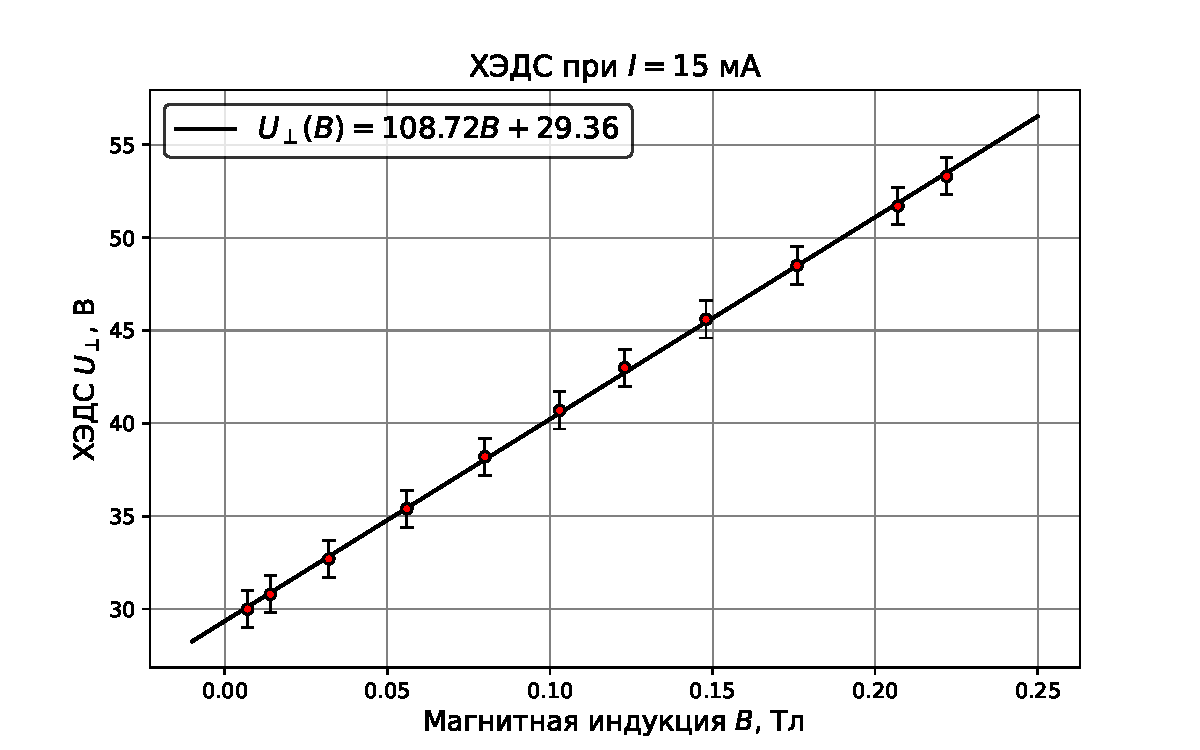
\includegraphics[scale=0.6]{Hall}
\end{center}

Из формулы (2): $\alpha=R\,\frac{I}{d}$, где $\alpha = 108,72\;\left( \frac{\mbox{В}}{\mbox{Тл}}\right)$ $\Rightarrow$ $R=\alpha\,\frac{d}{I}$
$$ R=108,72\cdot\frac{10^{-3}}{15\cdot10^{-3}}=7,248\;\left( \frac{\mbox{м}^3}{\mbox{Кл}}\right) $$

По формуле (3) находим концентрацию носителей заряда:
$$n=\frac{1}{1,6\cdot10^{-19}\cdot7,248}\approx8\cdot10^{17}\;(\mbox{м}^{-3})$$


	\end{document}
